\section{Entwurf des Data Warehouse}
\subsection{Relationale Umsetzung eines MDM-Schemas}
Zur Realisierung, der in Phase 1 entworfenen Data Cubes, sollen die nachfolgenden relationalen Modelle verwendet werden. Es wurde sich hierbei für das Star-Schema entschieden. Dieses bietet gegenüber dem Snowflake-Schema eine einfachere Struktur der Cubes und eine effizientere Anfrageverarbeitung durch die Vermeidung von JOIN-Operationen.  Die notwendigen Befehle zum Anlegen der Dimensions- und Faktentabelle sind in der beigefügten SQL-Datei zu finden. 

\subsubsection{Data Cube für die Anzahl der Bestellungen}
\begin{figure}[htbp] 
    \centering
       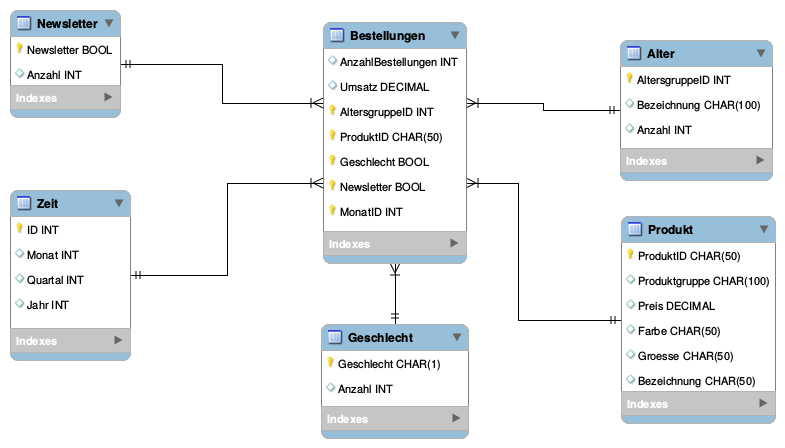
\includegraphics[width=0.8\textwidth]{phase2/dwh-bestellungen.png}
    \caption{Relationales Umsetzung des Cubes \textit{Bestellungen}}
    \label{fig:bestellungen}
  \end{figure} 
   
Der Data Cube \textit{Bestellungen} setzt sich aus der Faktentabelle \textit{Bestellungen} und den Dimensiontabellen \textit{Alter}, \textit{Produkt}, \textit{Geschlecht} und \textit{Zeit} zusammen.
\pagebreak

\subsubsection{Data Cube für die Anzahl der Retouren}
\begin{figure}[htbp] 
    \centering
       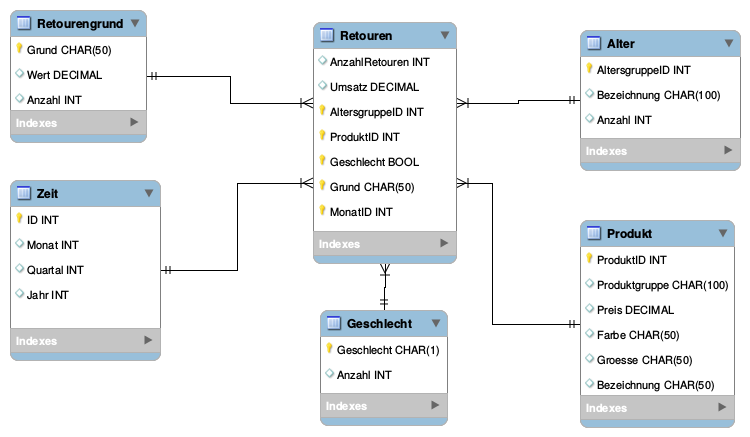
\includegraphics[width=0.8\textwidth]{phase2/dwh-retouren.png}
    \caption{Relationales Umsetzung des Cubes \textit{Retouren}}
    \label{fig:retouren}
\end{figure}  
Analog zum Cube \textit{Bestellungen} wurde auch der Data Cube \textit{Retouren} zur Analyse der Reklamationen in eine Faktentabelle und mehrere Dimensionstabellen untergliedert. 
  
  
\subsubsection{Data Cube für Cross-Sells}
\begin{figure}[htbp] 
    \centering
       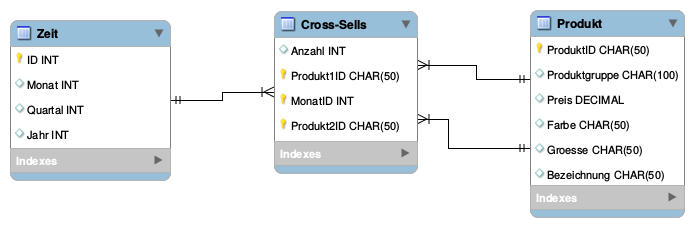
\includegraphics[width=0.72\textwidth]{phase2/dwh-cross.png}
    \caption{Relationales Umsetzung des Cubes \textit{Cross-Sells}}
    \label{fig:bestellungen}
  \end{figure}  
  
Mithilfe des Data Cubes \textit{Cross-Sells} soll, wie bereits erwähnt, untersucht werden, welche Produkte besonders häufig zusammen gekauft werden. Da zwischen den Produkten eine Art m-zu-n-Beziehung besteht, besitzt die Faktentabelle \textit{Cross-Sells} zwei Fremdschlüssel auf die Dimensionstabelle \textit{Produkt}.
  
\subsection{Optimierung der Data Cubes}
Zur Optimierung der Data Cubes stehen verschiedene Möglichkeiten zur Verfügung. So könnten durch materialisierte Sichten sowohl für die Cubes also auch für die Basis-Datenbank das Laden der Daten bzw. der Analyseprozess beschleunigt werden. Dabei wäre es ausreichend, wenn diese wöchentlich aktualisiert werden. Auch die Verwendung von Indexen wäre denkbar, um so die Abarbeitung bestimmter Analyseabfragen zu beschleunigen.